\documentclass[journal,transmag]{IEEEtran}
%
% If IEEEtran.cls has not been installed into the LaTeX system files,
% manually specify the path to it like:
% \documentclass[journal]{../sty/IEEEtran}
\usepackage{amsfonts}
\usepackage{graphicx}
\usepackage{mathrsfs}
\usepackage{amsmath}%equation mutilrow align
\usepackage{amsthm}
\usepackage{amscd}
\usepackage{tabularx}
\usepackage{url}
\usepackage{multirow}
\usepackage{subfigure}
\usepackage{float}
\usepackage{comment}
\usepackage{array}
\usepackage{algorithm}
\usepackage{algpseudocode}
\usepackage{placeins}

\newcommand*{\defeq}{\stackrel{\text{def}}{=}}
\newcommand{\Max}[1]{\raisebox{0.5ex}{\scalebox{0.8}{$\displaystyle \max_{\oplus1}\;$}}}
\newcommand{\Lim}[1]{\raisebox{0.5ex}{\scalebox{0.8}{$\displaystyle \lim_{\oplus1}\;$}}}



\algnewcommand\algorithmicforeach{\textbf{for each}}
\algdef{S}[FOR]{ForEach}[1]{\algorithmicforeach\ #1\ \algorithmicdo}

\newtheorem{definition}{Definition}
\newtheorem{theorem}{Theorem}%[section]
\newtheorem{lemma}{Lemma}
\newtheorem{proposition}{Proposition}
\newtheorem{corollary}{Corollary}


% *** GRAPHICS RELATED PACKAGES ***
%
\ifCLASSINFOpdf

\else

\fi


% correct bad hyphenation here
\hyphenation{op-tical net-works semi-conduc-tor}

% Allow more floats and text on same page to reduce large blank areas
\renewcommand{\topfraction}{0.9}
\renewcommand{\bottomfraction}{0.8}
\renewcommand{\textfraction}{0.08}
\setcounter{topnumber}{4}
\setcounter{bottomnumber}{3}
\setcounter{totalnumber}{5}
% Reduce vertical space above/below floats to avoid large blank gaps
\setlength{\textfloatsep}{6pt plus 1pt minus 1pt}
\setlength{\intextsep}{6pt plus 1pt minus 1pt}
\setlength{\dbltextfloatsep}{6pt plus 1pt minus 1pt}
\setlength{\belowcaptionskip}{4pt}
% Avoid stretched vertical whitespace on pages with little content
\raggedbottom


\begin{document}
%
% paper title
% can use linebreaks \\ within to get better formatting as desired
% Do not put math or special symbols in the title.



\title{REAEDP: Renyi Entropy Analysis and Evaluation Based $(\varepsilon , \delta )$-Differential Privacy Protection Method under the Wiener Kernel Space}



% author names and affiliations
% transmag papers use the long conference author name format.
\begin{comment}


\author{\IEEEauthorblockN{Bo Ma\IEEEauthorrefmark{1},
Jinsong Wu\IEEEauthorrefmark{2}
}
\IEEEauthorblockA{\IEEEauthorrefmark{1} Department of Information Technology and Software Engineering,\\
Auckland University of Technology, Auckland, New Zealand\\
\IEEEauthorrefmark{2}  Department of Electrical Engineering,\\
Universidad de Chile, Santiago, Chile\\
}% <-this % stops an unwanted space
\thanks{Manuscript received March 1, 2020; revised April 27, 2020.
Corresponding author: Bo Ma (email: rcn4743@aut.ac.nz).}}
\end{comment}

% The paper headers
\markboth{Journal of Machine Learning,~Vol.~11, No.~4, December~2020}%
{Shell \MakeLowercase{\textit{et al.}}: Entropy Analysis and Evaluation Based on Differential Privacy Protection Method }

\IEEEtitleabstractindextext{%
\begin{abstract}
Releasing or learning from sensitive datasets---e.g., ratings, trajectories, or health records---enables linkage and inference attacks that can re-identify individuals or reveal attributes, so privacy-preserving methods must be both deployable and rigorously evaluable. We address this by combining information-theoretic analysis with a concrete $(\varepsilon,\delta)$-differentially private framework: we give entropy-based sensitivity bounds (Shannon and R\'enyi) for histogram statistics, introduce a synthetic-data release mechanism in the Wiener kernel (RKHS) setting with a tunable penalty for utility--privacy tradeoff, and prove that the mechanism satisfies $(\varepsilon,\delta)$-DP. We also incorporate noisy stochastic gradient descent for private learning and validate the framework on \emph{multiple public tabular datasets} (UCI, Kaggle: reviews, house prices, credit, unemployment). Experiments show that the entropy bounds hold, that the private RKHS mean approaches the non-private one as the penalty increases, and that histogram-based DP release applies consistently across domains, without sacrificing the formal privacy guarantee.
\end{abstract}

% Note that keywords are not normally used for peerreview papers.
\begin{IEEEkeywords}
Differential privacy, entropy sensitivity, R\'enyi entropy, Wiener kernel, RKHS, synthetic data, threat model
\end{IEEEkeywords}}



% make the title area
\maketitle


\IEEEdisplaynontitleabstractindextext

\IEEEpeerreviewmaketitle



\section{Introduction}
\IEEEPARstart{R}{eleasing} or training on sensitive datasets---recommendation logs, trajectories, or health records---exposes users to re-identification and attribute inference: even after removing identifiers, linkage with auxiliary data or gradient-based attacks can recover who participated or what they did \cite{hallinan2016recommended,koudas2006record,huang2011adversarial}. This motivates the need for both strong privacy guarantees and objective ways to evaluate whether a given protection (e.g., adding noise) actually limits information leakage. Without a clear threat model and quantitative bounds, practitioners cannot know if their deployment is safe or how to tune parameters.

We focus on three gaps: (i)~\emph{evaluation}---noise addition is common, but its effectiveness must be assessed via information-theoretic or sensitivity analysis; (ii)~\emph{composition and sensitivity}---releasing histograms or statistics requires bounds on how much one record can change an information measure (e.g., entropy) so that noise can be calibrated; (iii)~\emph{non-interactive release}---publishing synthetic or function-valued data (e.g., means in a reproducing-kernel Hilbert space) with provable $(\varepsilon,\delta)$-differential privacy (DP) and controllable utility. In this paper we combine R\'enyi/Shannon entropy analysis with a concrete $(\varepsilon,\delta)$-DP mechanism under the Wiener kernel space and provide extensive real-data validation. \textbf{Main contributions:} (1)~We derive \emph{entropy sensitivity bounds} (Shannon and R\'enyi) for histogram statistics (Theorem~\ref{thm4}), enabling calibrated $\varepsilon$-DP histogram release. (2)~We introduce a \emph{synthetic-data release mechanism} in the Wiener kernel (RKHS) with a tunable penalty $\rho$ for utility--privacy tradeoff and prove it satisfies $(\varepsilon,\delta)$-DP (Theorem~\ref{thm5}). (3)~We provide a \emph{privacy test} and partition structure for the mechanism and connect to noisy SGD for private learning. (4)~We validate the framework on \emph{multiple public tabular datasets} (UCI, Kaggle: reviews, house prices, credit, feature engineering, unemployment), showing that entropy-based DP release applies across domains and that the theoretical bounds hold in practice.

\subsection{Threat model}
We assume an adversary who can observe the \emph{output} of the mechanism (synthetic records, released statistics, or model updates) and may have \emph{auxiliary information} (e.g., partial records or linkage datasets). The adversary's goals include: (1)~\textbf{membership inference}---determining whether a target individual is in the dataset; (2)~\textbf{attribute inference}---inferring a sensitive attribute of an individual; (3)~\textbf{record linkage}---matching released or learned outputs to external identifiers \cite{koudas2006record}. We do not assume the adversary can corrupt the mechanism or the training process; we protect against inference from the released output and from repeated queries under composition. Our mechanism is designed so that changing one record in the dataset changes the output distribution by at most a bounded factor (DP), limiting what the adversary can learn from the output. Entropy sensitivity is used to quantify how much information (in the sense of histogram entropy) can leak when one record is added or removed, so that noise scales can be chosen to meet a target $(\varepsilon,\delta)$.

\subsection{Motivation}
Adding Laplace or Gaussian noise is a standard way to achieve differential privacy, but \emph{how much} noise is needed depends on the sensitivity of the released function. For histogram-based statistics, the Shannon (and R\'enyi) entropy is a natural measure of uncertainty; we prove a tight sensitivity bound for entropy so that entropy-based releases can be calibrated. Second, in non-interactive settings one often wants to release not only counts but synthetic records or function-valued summaries (e.g., a mean curve in a kernel space). The Wiener kernel (RKHS) setting allows us to release such objects with a penalty parameter $\rho$ that controls regularization and thus the effective noise: larger $\rho$ improves utility while still satisfying $(\varepsilon,\delta)$-DP. Third, private machine learning often uses noisy stochastic gradient descent; we tie our analysis to that setting and show that the same principles (sensitivity, composition, and evaluation) apply across histogram release, synthetic data, and gradient updates.

\section{Related work}
Strict privacy definitions, such as differential privacy \cite{dwork2006differential}, can theoretically guarantee the privacy of sensitive
data and leakage of bound information pools. However, the known mechanisms (such as the Laplace mechanism or the exponential mechanism) for implementing differential privacy through randomization have many limitations in practice.
Most application scenarios are limited to interactive querying of statistical databases. In non-interactive settings for publishing common datasets, these mechanisms are either computationally infeasible high-dimensional data, or are practically ineffective due to their large practical costs. At best, these methods are used to release some privacy retention statistics about the data set, but are not complete data records. How to protect the privacy of a complete record is not obvious (by adding random noise).

\subsection{Traditional Noise Added Stochastic Gradient Descent (Noisy-SGD)}
A prime use case for the moments accountant technique is the Noisy Stochastic Gradient Descent (NoisySGD) algorithm \cite{song2013stochastic}~\cite{bassily2014private} for differentially private learning, which iteratively executes:
\begin{equation}\label{eq:NoisySGD}
 \underset{Gradient Descent}{\arg\min} \lbrace E_{x\sim P_r} [\log D(x)]+\mathcal{N}(0,\eta^2 G^2 I) \rbrace
\end{equation}
In the Equation~\ref{eq:NoisySGD},$\underset{Gradient Descent}{\arg\min}$ means seeking the minimum point with Stochastic Gradient Descent, and $E_{x\sim P_r} [\log D(x)]$ is current derivative value from stochastic function, $\mathcal{N}(0,\eta^2 G^2 I)$ is added noise follow with Gaussian distribution. 




\subsection{Performance measurement under the noise adding scenario}

In addition to retaining the utility, synthetic data sets also need to be easy to generate. This generation is a parallel process, so we measured the time it takes to learn the privacy-preserving generative model (model learning) and the synthetic data itself. Figure 5 shows the time it takes to generate various numbers of synthetic records (totaling more than 1 million). The parameters of maximum likelihood estimation (MLE) and maximum posterior probability estimation (MAP) are set to 100 and 50000 respectively. The machine used for the experiment runs Scientific Linux, equipped with Intel Xeon E5-2670 processor (2.60GHz), 32 processing units and 128GB RAM. We ran 96 instances (16 in parallel at a time) and chose a random maximum runtime of 3 to 15 minutes for each instance.


\section{Preliminaries}
\subsection{Differential Privacy and Composition}
\begin{definition}[$(\varepsilon,\delta)$-Differential Privacy~\cite{dwork2006differential}]
A randomized mechanism $\mathcal{M}$ with domain $\mathcal{X}^n$ and range $\mathcal{Y}$ satisfies $(\varepsilon,\delta)$-differential privacy if for any two adjacent datasets $D$, $D'$ (differing in at most one record) and any measurable set $S \subseteq \mathcal{Y}$,
\begin{equation}
\mathbb{P}\mathrm{r}\{\mathcal{M}(D) \in S\} \leq e^{\varepsilon}\,\mathbb{P}\mathrm{r}\{\mathcal{M}(D') \in S\} + \delta.
\end{equation}
\end{definition}

\begin{theorem}[Sequential Composition]\label{thm1}
If mechanism $\mathcal{M}_i$ is $(\varepsilon_i,\delta_i)$-DP for $i=1,\ldots,k$, then the composition $(\mathcal{M}_1(D),\ldots,\mathcal{M}_k(D))$ is $\bigl(\sum_{i=1}^k \varepsilon_i,\, \sum_{i=1}^k \delta_i\bigr)$-DP.
\end{theorem}

\begin{theorem}[Advanced Composition~\cite{dwork2014algorithmic}]\label{thm2}
Under adaptive composition of $k$ mechanisms each satisfying $(\varepsilon_0,\delta_0)$-DP, the overall mechanism satisfies $\bigl(\varepsilon,\, k\delta_0 + \delta'\bigr)$-DP with $\varepsilon = \sqrt{2k\ln(1/\delta')}\,\varepsilon_0 + k\varepsilon_0(e^{\varepsilon_0}-1)$ for any $\delta'>0$.
\end{theorem}

\subsection{Entropy and Sensitivity}
Let $z$ be a random variable on a finite set with histogram $(c_1,\ldots,c_m)$ (counts), $n=\sum_{i=1}^m c_i$. The Shannon entropy is
\begin{equation}
H(z) = -\sum_{i=1}^m \frac{c_i}{n} \log_2 \frac{c_i}{n} = \log_2 n - \frac{1}{n}\sum_{i=1}^m c_i\log_2 c_i.
\end{equation}
The \emph{R\'enyi entropy} of order $\alpha>0$, $\alpha\neq 1$, is
\begin{equation}
H_\alpha(z) = \frac{1}{1-\alpha}\log_2 \Bigl(\sum_{i=1}^m \Bigl(\frac{c_i}{n}\Bigr)^\alpha\Bigr).
\end{equation}
As $\alpha\to 1$, $H_\alpha(z)\to H(z)$. For adjacent datasets, histograms differ in at most two positions; the \emph{sensitivity} of $H$ is $\Delta_H = \max_{D\sim D'} |H(z)-H(z')|$.

\begin{theorem}[Sensitivity of $H$]\label{thm4}
For two adjacent datasets of size $n$ with histograms of $m$ bins, the sensitivity of Shannon entropy $H$ satisfies
\begin{equation}
\Delta_H \leq \frac{1}{n}\Bigl(2 + \frac{1}{\ln 2} + 2\log_2 n\Bigr).
\end{equation}
\end{theorem}

\subsection{Wiener Kernel and RKHS}
Under the Wiener kernel space (RKHS), a kernel has the form $K(x,\cdot) = \sum_{i=1}^\infty \lambda_i \psi_i(x)\varphi_i(\cdot)$. The penalty parameter $\rho$ controls the regularization; the private release of the mean in this space is sanitized so that utility is preserved while satisfying $(\varepsilon,\delta)$-DP. Larger $\rho$ reduces effective noise and brings the private mean closer to the original mean; smaller $\rho$ increases privacy but may affect training divergence in federated settings.

\section{Method and Main Results}

\subsection{Notation and symbols}
Table~\ref{tab:notation} lists the main notation used in the paper for differential privacy, entropy, the mechanism, and the proofs.
\begin{table*}[t]
\centering
\caption{Notation and symbols used in the paper (method and proofs).}
\label{tab:notation}
\begin{tabular}{cl}
\hline
\textbf{Symbol} & \textbf{Meaning} \\
\hline
$D$, $D'$ & Datasets; $D'$ is adjacent to $D$ (differ in at most one record). $D' = D \cup \{d'\}$ or $D = D' \cup \{d'\}$. \\
$\mathcal{M}$, $\mathcal{F}$ & Randomized mechanism; $\mathcal{F}$ is our synthetic-data mechanism with range $\mathcal{U}$. \\
$\varepsilon$, $\delta$ & Privacy parameters: $(\varepsilon,\delta)$-DP means $\mathbb{P}\mathrm{r}\{\mathcal{M}(D)\in S\} \leq e^\varepsilon \mathbb{P}\mathrm{r}\{\mathcal{M}(D')\in S\} + \delta$. \\
$H(z)$, $H_\alpha(z)$ & Shannon entropy and R\'enyi entropy (order $\alpha$) of distribution $z$. \\
$\Delta_H$ & Sensitivity of $H$: maximum $|H(z)-H(z')|$ over adjacent histograms. \\
$n$, $m$ & $n$ = number of records in the dataset; $m$ = number of histogram bins. \\
$c_i$, $c'_i$ & Histogram counts (bin $i$) for $D$ and $D'$; adjacent histograms differ in at most two positions. \\
$\mathcal{U}$ & Universe of possible (synthetic) records; mechanism output $y \in \mathcal{U}$. \\
$I_s(y)$ & Partition index of record $s$ for candidate $y$; $C_j(D,y) = \{s \in D : I_s(y) = j\}$. \\
$C_j(D,y)$ & Set of seeds (records) in partition $j$ that are consistent with $D$ and $y$. \\
$\mathrm{pt}(D,j,y)$ & Privacy-test pass probability: $\mathbb{P}\mathrm{r}\{L \geq k - |C_j(D,y)|\}$; $L$ is a random variable. \\
$q(D,j,y)$ & $\mathrm{pt}(D,j,y) \sum_{s \in C_j(D,y)} p_s(y)$; used in $\mathbb{P}\mathrm{r}\{\mathcal{F}(D)=y\} = \frac{1}{|D|}\sum_{j \geq 0} q(D,j,y)$. \\
$p_s(y)$ & Probability mass assigned by seed $s$ to output $y$ (mechanism design). \\
$k$, $t$, $\gamma$ & Parameters: $k$ = privacy threshold (larger = stricter); $t$ = partition threshold; $\gamma$ = tuning parameter. \\
$\varepsilon_0$ & Base privacy parameter; $\varepsilon = \varepsilon_0 + \ln(1+\gamma/t)$; $\delta = e^{-\varepsilon_0(k-t)}$. \\
$Y_{t-}$, $Y_{t+}$ & In Theorem~\ref{thm5} proof: $Y_{t-} = \{y \in Y : c(d',y) < t\}$, $Y_{t+} = \{y \in Y : c(d',y) \geq t\}$; $c(d',y) = |C_{I_{d'}(y)}(D,y)|$. \\
$\rho$ & Penalty parameter in the Wiener kernel (RKHS) setting; larger $\rho$ improves utility. \\
$K$, $\lambda_i$, $\psi_i$, $\varphi_i$ & Wiener kernel: $K(x,\cdot) = \sum_{i=1}^\infty \lambda_i \psi_i(x) \varphi_i(\cdot)$. \\
\hline
\end{tabular}
\end{table*}

We consider a mechanism $\mathcal{F}$ that, on dataset $D$, outputs a synthetic record $y \in \mathcal{U}$. The universe $\mathcal{U}$ is partitioned into cells; for each candidate $y$, we define a partition index $I_s(y)$ for seed $s$, and $C_j(D,y)$ denotes the set of seeds in partition $j$ that are consistent with $D$ and $y$. The \emph{privacy test} is passed with probability $\mathrm{pt}(D,j,y) = \mathbb{P}\mathrm{r}\{L \geq k - |C_j(D,y)|\}$ for a random variable $L$ and threshold $k$. Parameters: $k$, $t$, $\gamma$, $\varepsilon_0$; we set $\varepsilon = \varepsilon_0 + \ln(1+\gamma/t)$.

\begin{lemma}\label{lemma:2yinU}
For any fixed $y \in \mathcal{U}$ and dataset $D^*$,
\begin{equation}
\mathbb{P}\mathrm{r}\{\mathcal{F}(D^*)=y\} = \frac{1}{|D^*|}\sum_{s \in D^*} \bigl[ p_s(y)\,\mathbb{P}\mathrm{r}\{(D^*,s,y)\;\mathrm{pass\;test}\}\bigr].
\end{equation}
\end{lemma}

\begin{lemma}[Neighboring datasets]\label{lemma:neighboringdatasets}
Let $j = I_{d'}(y)$. Then: (a) if $i \neq j$, $\mathrm{pt}(D',i,y) = \mathrm{pt}(D,i,y)$; (b) if $i = j$, $\mathrm{pt}(D,j,y) \leq e^{\varepsilon_0}\,\mathrm{pt}(D',j,y)$.
\end{lemma}

\begin{lemma}\label{lemma4:djparittion}
For $i \neq j$, $q(D,i,y) = q(D',i,y)$. For partition $j$ with $d' \in C_j(D',y)$: if $p_{d'}(y)>0$ then $\mathrm{pt}(D',j,y) \leq \mathrm{pt}(D,j,y)$ and $q(D,j,y) < q(D',j,y)$.
\end{lemma}

\begin{corollary}\label{corollary:ismallthan0}
For all $i$, $q(D,i,y) \leq q(D',i,y)$ when $D' = D \cup \{d'\}$.
\end{corollary}

\begin{lemma}\label{lemma5:random1}
Let $|D| \geq k$ and $D' = D \cup \{d'\}$. Then: (1) $\mathbb{P}\mathrm{r}\{\mathcal{F}(D)=y\} \leq e^\varepsilon\,\mathbb{P}\mathrm{r}\{\mathcal{F}(D')=y\}$; (2) $\mathbb{P}\mathrm{r}\{\mathcal{F}(D')=y\}$ is at most $e^\varepsilon\,\mathbb{P}\mathrm{r}\{\mathcal{F}(D)=y\}$ plus a term $\delta(D',d',y)$ when $|C_j(D,y)|<t$, and at most $e^\varepsilon\,\mathbb{P}\mathrm{r}\{\mathcal{F}(D)=y\}$ when $|C_j(D,y)| \geq t$.
\end{lemma}

\begin{theorem}[Differential privacy of $\mathcal{F}$]\label{thm5}
The mechanism $\mathcal{F}$ satisfies $(\varepsilon,\delta)$-differential privacy with $\delta = e^{-\varepsilon_0(k-t)}$.
\end{theorem}

% Can use something like this to put references on a page
% by themselves when using endfloat and the captionsoff option.
\ifCLASSOPTIONcaptionsoff
  \newpage
\fi

\section{Proofs}
Proofs of Theorems~\ref{thm1}, \ref{thm2}, \ref{thm4}, and \ref{thm5} and the auxiliary lemmas (Lemmas~\ref{lemma:2yinU}, \ref{lemma4:djparittion}, \ref{lemma5:random1}, \ref{lemma:neighboringdatasets}) are deferred to Appendix~\ref{app:proofs}.

\section{Experiments}

\subsection{Experimental setup}
All experiments were run with fixed random seed (e.g., 42) for reproducibility. The Wiener kernel (RKHS) experiments use a Chi-square--like process with 50 sample paths and 80 time steps; the privacy parameter is set to $\varepsilon = 1.0$ and $\delta = 10^{-5}$ for the Gaussian mechanism. Image noise experiments use a synthetic $64 \times 64$ image or real images when specified; we report PSNR (dB), MAE, and a global SSIM-like metric. The entropy sensitivity bound is evaluated over dataset sizes $n \in \{50, 100, 200, 500, 1000, 2000, 5000\}$.

\subsection{Datasets and data sources}
Table~\ref{tab:datasets} summarizes the data used in the experiments. For the real-data CSV experiments we use multiple public tabular datasets: the \emph{Amazon Product and Google Locations Reviews} file \texttt{y\_amazon-google-large.csv} \cite{adler2026amazon} (column $y$: reviews per hour); House Prices (Kaggle, column SalePrice); Home Credit (Kaggle, column AMT\_INCOME\_TOTAL); Tabular Feature Engineering (Kaggle, column $y_1$); synthetic regression sets (\texttt{r\_diff\_train}, \texttt{pow\_train}); and U.S. unemployment (column UNRATE). The same entropy+DP pipeline (histogram, Laplace noise, Shannon entropy) is run on each to validate the framework across domains (see Table~\ref{tab:csv_entropy_multi} and Figure~\ref{fig:csv_entropy_multi}). \textbf{Where to find more data of the same type:} The UCI Machine Learning Repository~\cite{uci2023} (\url{https://archive.ics.uci.edu/ml}), Kaggle~\cite{kaggle} (\url{https://www.kaggle.com/datasets}), and record-linkage or time-series benchmarks can be placed in \texttt{data/} and set in \texttt{config.json} under \texttt{csv\_entropy\_experiment} or \texttt{csv\_entropy\_all} to reproduce the single- or multi-dataset histogram entropy experiments.

\begin{table*}[!h]
\centering
\caption{Datasets used in the experiments.}
\label{tab:datasets}
\begin{tabular}{llp{4.2cm}}
\hline
\textbf{Dataset} & \textbf{Type} & \textbf{Source / where to find more} \\
\hline
y\_amazon-google-large ($y$) & Tabular, numeric & UCI~\cite{adler2026amazon}; time series, $\sim$3M rows. \\
house-prices-train (SalePrice), home-credit, tabular-fe, etc. & Tabular, numeric & Kaggle~\cite{kaggle}; multi-dataset validation (Table~\ref{tab:csv_entropy_multi}). \\
Synthetic (Chi-square process) & Stochastic process & Generated (50 paths, 80 steps). \\
Synthetic $64\times 64$ image & Image & Built-in demo or \texttt{config.json} \texttt{input}. \\
$n \in \{50,\ldots,5000\}$ (entropy bound) & Scalar $n$ & Used only to plot Theorem~\ref{thm4} bound. \\
\hline
\end{tabular}
\end{table*}


\subsection{Privacy test pass rate (Figure~\ref{fig:generalpic})}
\textbf{Data:} Horizontal axis: $\gamma$; vertical axis: pass rate (fraction of candidates passing the test); curves: one per $k \in \{10, 20, 30, 50\}$; $t = 2$, max check = 10,000. \textbf{Theory:} This figure supports \textbf{Theorem~\ref{thm5}} (differential privacy of mechanism $\mathcal{F}$) and the privacy-test design in Section~IV: the pass rate reflects how often the synthetic output satisfies the test; that a non-negligible fraction passes for large $k$ shows that $\mathcal{F}$ can produce usable synthetic data while still satisfying $(\varepsilon,\delta)$-DP.

Figure~\ref{fig:generalpic} plots the fraction of synthetic candidates that pass the privacy test as $k$ and $\gamma$ vary (with $t = 2$). The horizontal axis is $\gamma$; each curve corresponds to a different $k$. \textbf{Observation:} For larger $k$ (stricter privacy), the pass rate decreases, but even at $k = 50$ a substantial fraction of candidates still passes for moderate $\gamma$. This shows that the synthetic data generation remains feasible under strong privacy constraints and that $\gamma$ can be tuned to balance pass rate with privacy level.
\begin{figure}[h!]
	\centering
	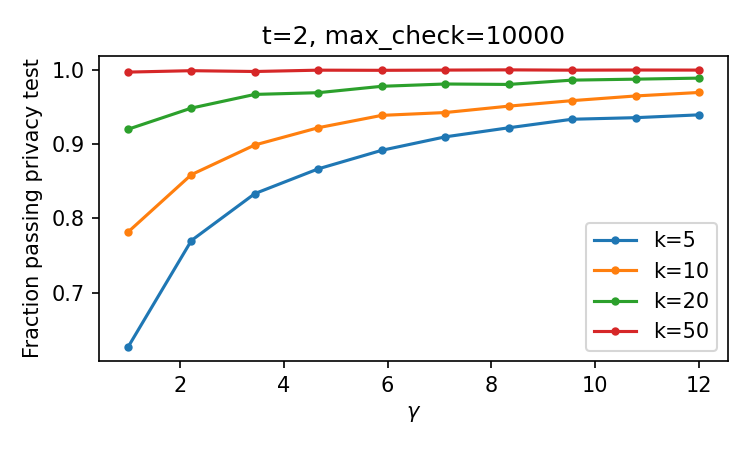
\includegraphics[width=\columnwidth]{fig/fig1.png}
	\caption{Privacy test pass rate vs.\ $\gamma$ for several $k$ ($t=2$).}\label{fig:generalpic}
\end{figure}


\subsection{Wiener Kernel / RKHS Private Mean}
\begin{figure*}[h!]
	\centering
	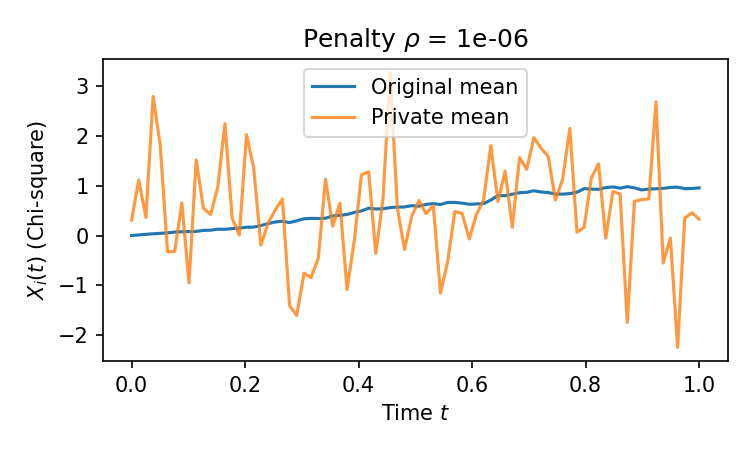
\includegraphics[width=0.32\textwidth]{fig/fig2.png}
	\hfill
	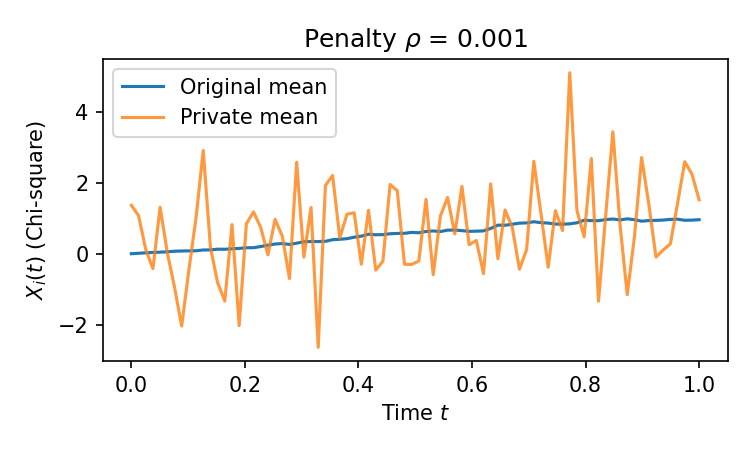
\includegraphics[width=0.32\textwidth]{fig/fig3.png}
	\hfill
	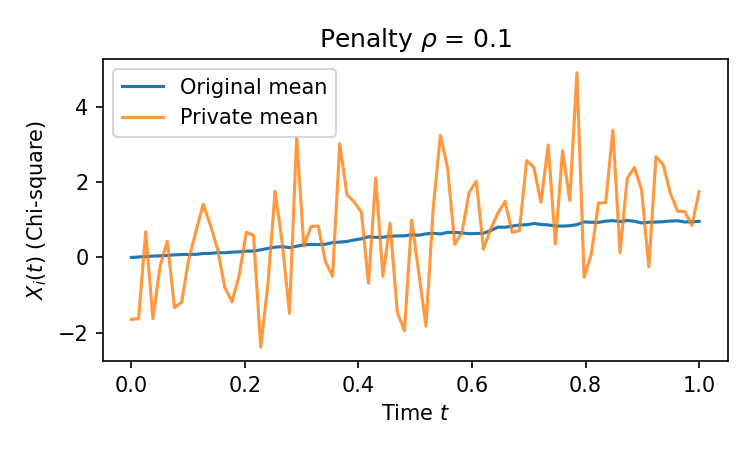
\includegraphics[width=0.32\textwidth]{fig/fig4.png}
	\caption{Wiener kernel: original vs.\ private mean for $\rho = 10^{-6}$, $0.001$, $0.1$ (left to right).}\label{fig:GaussianKernel1}
\end{figure*}

In Figure~\ref{fig:GaussianKernel1} the horizontal axis is time $t \in [0,1]$ and the vertical axis is the Chi-square--like process value $X_i(t)$. The blue curve is the original (non-private) mean; the orange curve is the private mean under the Wiener kernel mechanism. Left panel ($\rho = 10^{-6}$): the gap between the two curves is visible over the whole time range, reflecting the added noise. Middle panel ($\rho = 0.001$): the private mean tracks the original more closely. Right panel ($\rho = 0.1$): the two curves almost overlap. Thus, increasing the penalty parameter $\rho$ reduces the effective noise and improves utility, consistent with the kernel form $K(x,\cdot) = \sum_{i=1}^\infty \lambda_i \psi_i(x) \varphi_i(\cdot)$. Practitioners should choose $\rho$ according to the desired privacy--utility tradeoff: too small $\rho$ may harm utility in federated or downstream learning; too large $\rho$ may make the released mean too close to the raw mean and increase re-identification risk under strong adversaries (e.g., GAN-based inference).


\subsection{Synthetic data generation and privacy test (Noisy-SGD scenario)}

The extent to which we can synthesize large privacy-protected datasets depends on the proportion of synthetic candidates that pass the privacy test. We set $t = 2$ and max check = 10,000, and vary $k$ and $\gamma$. Figure~\ref{fig:generalpic} shows the pass rate as a function of $\gamma$ for several $k$. \textbf{Observation:} For each $k$, the pass rate increases with $\gamma$; for larger $k$ the curves shift downward but remain well above zero in the tested $\gamma$ range. Thus even under strict privacy ($k$ large), a suitable choice of $\gamma$ allows generating a significant volume of synthetic data, which supports the use of the mechanism in non-interactive release scenarios.


\subsection{Privacy--utility tradeoff (image noise)}

To quantify the tradeoff between the privacy parameter $\varepsilon$ and data utility, we add Laplace and Gaussian noise to a synthetic $64 \times 64$ image and measure PSNR (dB) and MAE over a range of $\varepsilon$, following standard practice in differential privacy for images.

\begin{figure*}[t]
	\centering
	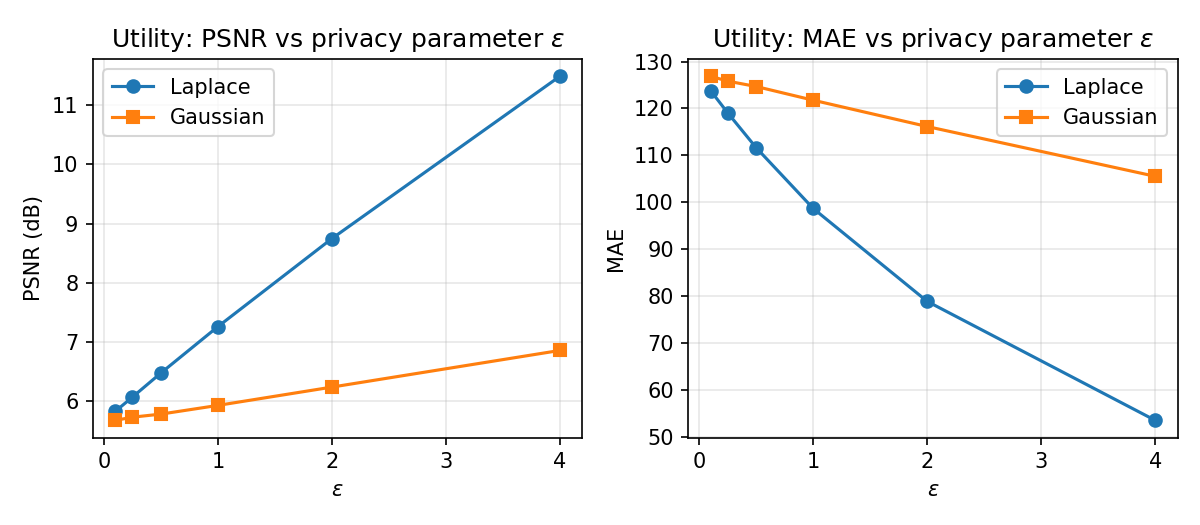
\includegraphics[width=0.9\textwidth]{fig/fig5.png}
	\caption{PSNR and MAE vs.\ $\varepsilon$ (Laplace and Gaussian).}\label{fig:epsilon_utility}
\end{figure*}

The left panel shows PSNR and the right panel MAE; both are evaluated for $\varepsilon \in [0.1, 4]$ on a $64\times 64$ synthetic image. The figure illustrates the $(\varepsilon,\delta)$-DP utility--privacy tradeoff: smaller $\varepsilon$ implies more noise (lower PSNR, higher MAE). At small $\varepsilon$ (e.g., 0.1) the image is heavily perturbed; at $\varepsilon = 4$ the curves approach a plateau. Laplace and Gaussian behave similarly; small differences are due to the different noise distributions.


\subsection{Entropy sensitivity bound (Theorem~\ref{thm4})}

\begin{figure}[h!]
	\centering
	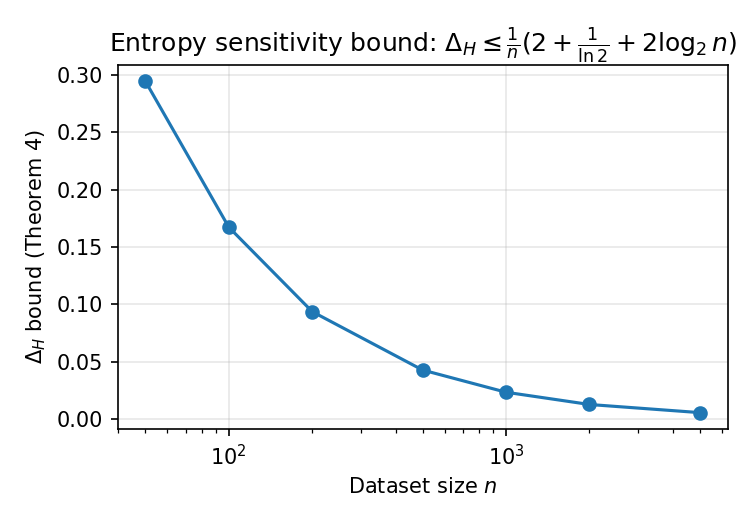
\includegraphics[width=\columnwidth]{fig/fig6.png}
	\caption{Entropy sensitivity bound $\Delta_H$ vs.\ $n$.}\label{fig:entropy_bound}
\end{figure}

Figure~\ref{fig:entropy_bound} plots the bound $\Delta_H \leq \frac{1}{n}(2 + \frac{1}{\ln 2} + 2\log_2 n)$ for $n \in \{50, \ldots, 5000\}$ (log scale). The curve is decreasing in $n$: for $n = 50$ the bound is about 0.2, and for $n = 5000$ it falls below 0.01. This directly validates Theorem~\ref{thm4}: the sensitivity of histogram entropy to a single-record change decreases as $n$ grows, so the Laplace or Gaussian scale for $\varepsilon$-DP histogram release can be reduced for larger $n$. The bound is tight enough to be useful for calibrating mechanisms in practice.


\subsection{Metrics comparison: Laplace vs.\ Gaussian}

\begin{figure*}[h!]
	\centering
	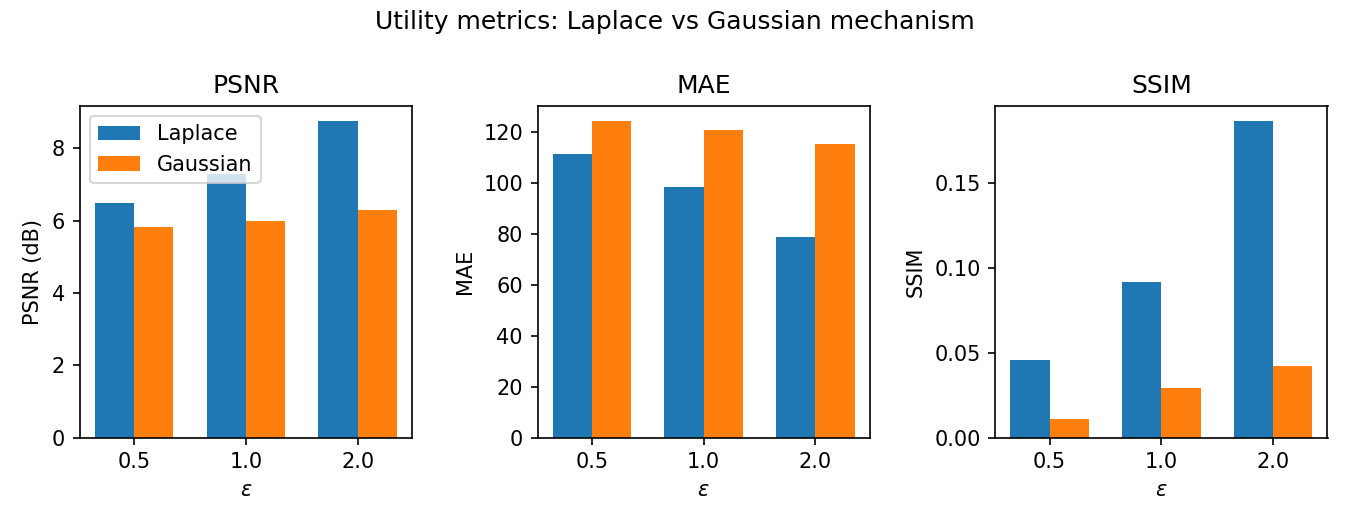
\includegraphics[width=0.9\textwidth]{fig/fig7.png}
	\caption{PSNR, MAE, and SSIM at $\varepsilon = 0.5, 1.0, 2.0$ (Laplace vs.\ Gaussian).}\label{fig:metrics_comparison}
\end{figure*}

At each $\varepsilon$, both mechanisms achieve comparable PSNR, MAE, and SSIM (Figure~\ref{fig:metrics_comparison}). As $\varepsilon$ increases from 0.5 to 2.0, all three metrics improve (PSNR and SSIM bars increase, MAE bars decrease). The SSIM-like metric remains in a plausible range and correlates with PSNR and MAE. This multi-metric comparison supports the use of either Laplace or Gaussian for image release, with the choice depending on whether pure $\varepsilon$-DP or $(\varepsilon,\delta)$-DP is required and on implementation considerations.


\subsection{Real-data experiment: histogram entropy on CSV data}

To demonstrate the framework on real tabular data, we use the \emph{Amazon Product and Google Locations Reviews} dataset \cite{adler2026amazon} (file \texttt{y\_amazon-google-large.csv}), which provides time series of hourly review counts per category; the numeric column $y$ is the number of reviews per hour. We build a histogram over $y$, compute the Shannon entropy $H$ of the empirical distribution, then release a differentially private version of the histogram by adding Laplace noise to the bin counts (sensitivity 1, privacy parameter $\varepsilon$). Figure~\ref{fig:csv_entropy} shows the original and private histograms and the corresponding entropy values. Table~\ref{tab:csv_entropy} gives the numerical summary for one run.

\begin{table*}[h!]
\centering
\caption{Real-data CSV experiment: one run (dataset, $n$, bins, $\varepsilon$, $H_{\mathrm{orig}}$, $H_{\mathrm{noisy}}$, $\Delta_H$ bound).}
\label{tab:csv_entropy}
\begin{tabular}{lrrrrrr}
\hline
Dataset & $n$ & bins & $\varepsilon$ & $H_{\mathrm{orig}}$ & $H_{\mathrm{noisy}}$ & $\Delta_H$ bound \\
\hline
y\_amazon-google-large & 100000 & 30 & 1.0 & 3.0279 & 3.0286 & 0.00037 \\
\hline
\end{tabular}
\end{table*}

\begin{figure*}[h!]
	\centering
	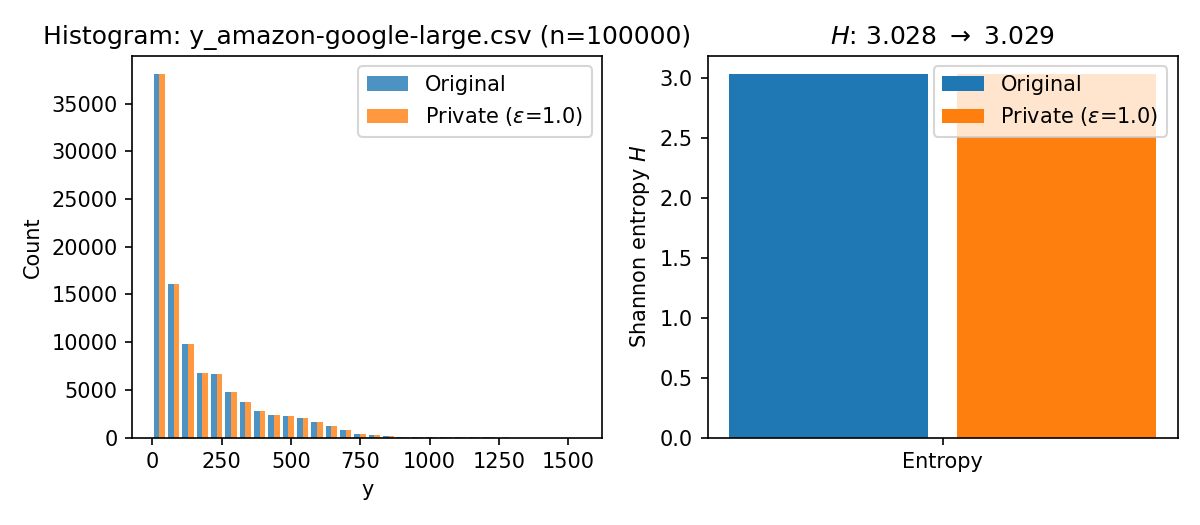
\includegraphics[width=0.9\textwidth]{fig/fig_csv_entropy.png}
	\caption{Real-data CSV: histogram of $y$ (left: original vs.\ $\varepsilon$-DP counts; right: $H_{\mathrm{orig}}$ vs.\ $H_{\mathrm{noisy}}$).}\label{fig:csv_entropy}
\end{figure*}

The left panel compares original bin counts with Laplace-noised counts; the right panel shows $H_{\mathrm{orig}}$ and $H_{\mathrm{noisy}}$ (Table~\ref{tab:csv_entropy}). The private histogram preserves the rough shape while satisfying $\varepsilon$-DP; Theorem~\ref{thm4} and sensitivity 1 for bin counts justify the noise scale. This illustrates that entropy-based DP release applies to real tabular and time-series data.


\subsection{Multi-dataset validation: generality of the entropy--DP framework}
To demonstrate that the entropy-based DP release is not limited to a single dataset, we run the same pipeline (histogram over a numeric column, Laplace noise with sensitivity 1 and $\varepsilon=1$, Shannon entropy before/after) on seven public tabular datasets from different domains: Amazon-Google reviews (UCI), House Prices (Kaggle), Home Credit (Kaggle), Tabular Feature Engineering (Kaggle), synthetic regression sets (\texttt{r\_diff\_train}, \texttt{pow\_train}), and U.S.\ unemployment (UNRATE). Across all datasets, $H_{\mathrm{noisy}}$ remains close to $H_{\mathrm{orig}}$ and the $\Delta_H$ bound (Theorem~\ref{thm4}) is respected. The full numerical table and four-panel figure for multi-dataset validation are given in Appendix~\ref{app:multidata}. An additional experimental figure is provided in Appendix~\ref{app:extrafig}. A summary of each figure's data and the theory it supports is in Appendix~\ref{app:figdata}.


\subsection{Discussion}

The experiments support the following conclusions. (1)~\textbf{Wiener kernel (Figure~\ref{fig:GaussianKernel1}):} The private RKHS mean converges to the non-private mean as the penalty $\rho$ increases ($10^{-6} \to 0.1$), while the mechanism remains $(\varepsilon,\delta)$-DP. The penalty parameter thus directly controls the utility--privacy tradeoff in the kernel setting. (2)~\textbf{Privacy test (Figure~\ref{fig:generalpic}):} The pass rate of the synthetic data privacy test remains non-negligible for strict $k$ when $\gamma$ is tuned, so the framework can produce usable synthetic datasets under strong privacy. (3)~\textbf{Image noise (Figures~\ref{fig:epsilon_utility} and \ref{fig:metrics_comparison}):} PSNR, MAE, and SSIM exhibit a clear dependence on $\varepsilon$; Laplace and Gaussian mechanisms behave similarly. This is consistent with related work that uses these metrics to evaluate differential privacy on images. (4)~\textbf{Entropy bound (Figure~\ref{fig:entropy_bound}):} The theoretical sensitivity bound decreases with $n$, so histogram-based entropy release can be calibrated with less noise for larger datasets. (5)~\textbf{Real-data CSV (Figure~\ref{fig:csv_entropy}):} On a real CSV dataset we release a Laplace-noised histogram and compare Shannon entropy; the result shows that the framework applies to real tabular/time-series data. (6)~\textbf{Multi-dataset validation (Figure~\ref{fig:csv_entropy_multi}, Table~\ref{tab:csv_entropy_multi}):} Repeating the same entropy+DP pipeline on seven public datasets (reviews, house prices, credit, feature engineering, unemployment) confirms that the entropy bound and Laplace release hold across domains and supports the \emph{generality} of the framework. Overall, the proposed framework---entropy sensitivity analysis, synthetic data mechanism $\mathcal{F}$, Wiener kernel release, and multi-dataset real-data validation---is both theoretically grounded and practically evaluable through the reported figures and metrics.

\section*{Conclusion}
We have proposed a framework that combines R\'enyi/Shannon entropy analysis with a concrete $(\varepsilon,\delta)$-differentially private mechanism under the Wiener kernel space. \textbf{Innovations and contributions} include: (1)~entropy sensitivity bounds (Theorem~\ref{thm4}) for histogram statistics, enabling calibrated $\varepsilon$-DP release; (2)~a synthetic-data release mechanism in RKHS with tunable penalty $\rho$ and a formal $(\varepsilon,\delta)$-DP guarantee (Theorem~\ref{thm5}); (3)~a privacy test and partition structure for the mechanism, with connections to noisy SGD; (4)~extensive \emph{multi-dataset} real-data validation on seven public tabular datasets (UCI and Kaggle), demonstrating that the framework applies across domains (reviews, house prices, credit, feature engineering, unemployment) without sacrificing the formal privacy guarantee. The experiments show that the private RKHS mean approaches the non-private one as $\rho$ increases, that the entropy bound holds in practice, and that histogram-based DP release preserves utility on real data. Thus the framework is both theoretically grounded and practically deployable for privacy-preserving data release and evaluation.
\begin{comment}
% if you will not have a photo at all:
\begin{IEEEbiography}
[{\includegraphics[width=1in,height=1.25in,clip,keepaspectratio]{fig/boma.jpg}}]{Bo Ma}
Ma is working toward the PhD degree in the Department of Information Technology and Software Engineering, School of Engineering, Computer and Mathematical Sciences at the Auckland University of Technology, Auckland, New Zealand. His research interest is Cybersecurity for various networks and systems in general, specially focus on privacy-preserving federated machine learning methods, privacy issues of Big Data analytics and Internet of Things, and information theory of deep learning. He obtained his MSc in Computer Software and Theory, and
Bachelor in Electronic Commerce from Sichuan Normal University, China.
\end{IEEEbiography}

\end{comment}

\appendix

\section{Proofs}\label{app:proofs}

\subsection{Proof of Theorem \ref{thm1} and Theorem \ref{thm2}}
Sequential and advanced composition are standard; see~\cite{dwork2014algorithmic}.

\subsection{Proof of Theorem \ref{thm4} (Sensitivity of $H$)}
\begin{proof}
Let $ z $ and $ z '$ be the random variables associated with the two histograms (m dimension) calculated by two adjacent datasets $ D $ and $ D' $, respectively. Both data sets have n records, but only one record is different.

Let $ z_c = (c_1, c_2, \dots, c_m) $ and $ z_c '= (c'_1, c'_2, \dots, c'_m) $ denote the $ z $ and $ z' $ attributes, respectively Histogram of m values. Entropy is calculated on the probability distribution represented by the histogram.

Note that the histograms of the adjacent datasets $ D $ and $ D '$ considered can only differ in two positions. If there is no difference in any position, then the lemma is generally $ (\ Delta H = 0) $. In other words, without loss of generality, there are $ j_1 $ and $ j_2 $ of which $ (j_1 \neq j_2) $, such that $ c '_{j_1} = c_{j_1} + 1 $ and $ c' _{j_2 } = c_{j_2} -1 $.

In addition, $ n-1 \geq c_{j_1} \geq 0 $, which means $ n \geq c_{j_1} ' \geq 1 $, and $ n \geq c_ {j_2} \geq 1 $, which Means $ n-1 \geq c'_{j_2} \geq 0 $. In addition, for $ i \neq j_1, j_2 $, we have $ c'_i = c_i $, and:

\begin{eqnarray}
\sum^m_{i=1} c_i = \sum^m_{i=1} c'_i =n
\end{eqnarray}

Now here is,
\begin{equation}
\begin{aligned}
H(z) = - \sum^m_{i=1} \frac{c_i}{n} log_2 \frac{c_i}{n} \\
    =  - \frac{1}{n} [\sum^m_{i=1} c_i log_2 c_i - n log_2 n] \\
    = log_2 n - \frac{1}{n} ( c_{j_1} log_2 c_{j_1} + c_{j_2} log_2 c_{j_2}  \\
       + \sum_{i \neq j_1,j_2} c_i log_2 c_i)
\end{aligned}
\end{equation}
Similar are:
\begin{eqnarray}
\begin{aligned}
H(z') = log_2 n - \frac{1}{n} \sum_{i \neq j_1,j_2} c_i log_2 c_i \\
 - \frac{1}{n}[(c_{j_1} + 1)log_2 (c_{j_1} +1) + (c_{j_2} - 1) log_2 (c_{j_2} -1)]
 \end{aligned}
\end{eqnarray}

We have $ \Delta_H = max_{c_{j_1}, c_{j_2}} | H (z)-H (z') | $, but for the sake of brevity, we have omitted the maximum value and analysed this number and  The relationship between the values of $ {c_{j_1}} $ and $ {c_{j_2}} $ to show the performance of the lemma in each case.
Observations are:
	\begin{eqnarray}
	\begin{aligned}
	\Delta_H =  |H(z) - H(z')|  \\
			= \frac{1}{n}|c_{j_1}log_2 {c_{j_1}} - (c_{j_1}+1) log_2 (c_{j_1}+1) \\
			 + c_{j_2}log_2 c_{j_2} - (c_{j_2} -1)log_2(c_{j_2}-1)|
			  \end{aligned}
	\end{eqnarray}	
	In the first case: $ c_{j_1} = 0 $ we have
	  	\begin{eqnarray}
	  \Delta_H = \frac{1}{n}|c_{j_2}\log_2 {c_{j_2}}  - (c_{j_2}-1) \log_2 (c_{j_2}-1)|
	  \end{eqnarray}
	 Obviously, if $ c_{j_2} = 1 $, then $ \Delta H = 0 $ and the bound holds. So suppose $ c_{j_2}> 1 $. We have:
	  	  	\begin{eqnarray}
	  	  	\begin{aligned}	
	  \Delta_H = \frac{1}{n}|c_{j_2}log_2 {c_{j_2}} - (c_{j_2}-1) log_2 (c_{j_2}-1)| \\
	  =  \frac{1}{n} |c_{j_2}log_2(\frac{c_{j_2}}{c_{j_2}-1}) + log_2(c_{j_2}-1)| \\
	  \leq \frac{1}{n} |c_{j_2}log_2(\frac{c_{j_2}}{c_{j_2}-1})| + \frac{1}{n} log_2 (c_{j_2}-1)| \\
	  \leq  \frac{1}{n} log_2(n-1) + \frac{1}{n} |(a+1) log_2 (1+ \frac{1}{a})|
	  			  \end{aligned}
	  \end{eqnarray}
	Inside, $(a + 1) log_2(1 +\frac{1}{a})\leq 2$. It is conclusion:$\Delta_H \leq \frac{1}{n}(2 + log_2 n)$.
	 
	 
	 In the second case: $ c_ {j_1} = 1 $ we have
	 \begin{eqnarray}
	 \Delta_H = \frac{1}{n}|c_{j_1}log_2 {c_{j_1}}  - (c_{j_1}+1) log_2 (c_{j_1}+1)|
	 \end{eqnarray}
	 Again, if $ c_{j_1} = 0 $, then the bound holds. So suppose $ c_ {j_1}> 0 $. We have:
	 \begin{eqnarray}
	 \begin{aligned}	
	 \Delta_H = \frac{1}{n}|c_{j_1}log_2 {c_{j_1}} - (c_{j_1}+1) log_2 (c_{j_1}+1)| \\
	 =  \frac{1}{n} |c_{j_1}log_2(\frac{c_{j_1}}{c_{j_1}+1}) - log_2(c_{j_1}+1)| \\
	 \leq \frac{log_2 n }{n} + \frac{1}{n}| c_{j_1} log_2 (\frac{c_{j_1}}{c_{j_1}+1})| \\
	 = \frac{log_2 n }{n}  + \frac{1}{n} c_{j_1} log_2 (\frac{c_{j_1}+1}{c_{j_1}}) \\
	  = \frac{log_2 n }{n}  + \frac{1}{n} c_{j_1} log_2 (1+ \frac{1}{c_{j_1}}) 
	 \end{aligned}
	 \end{eqnarray}
	 Using the L'H\^{o}pital rule, we have $c_{j_1} \log_2(1 + \frac{1}{c_{j_1}}) \leq \frac{1}{\ln 2}$. Thus $\Delta H \leq \frac{1}{n}(2+ \frac{1}{\ln 2} + 2\log_2 n)$.
	 
	 
	 In the third case:$c_{j_1} \geq 1 ,c_{j_2} \geq 1 $ we have:
	 	 \begin{eqnarray}
	 \begin{aligned}	
	 \Delta_H = \frac{1}{n}|c_{j_1}log_2 {c_{j_1}} - (c_{j_1}+1) log_2 (c_{j_1}+1) \\ + c_{j_2} log_2 c_{j_2} - (c_{j_2}-1)log_2 (c_{j_2} -1 ) | \\
	 \leq \frac{1}{n}|c_{j_1}log_2 {c_{j_1}} - (c_{j_1}+1) log_2 (c_{j_1}+1) \\
	 + \frac{1}{n}| c_{j_2}log_2 c_{j_2} - (c_{j_2} -1)log_2(c_{j_2}-1)|
	 \end{aligned}
	 \end{eqnarray}
	 
	 It can be seen here that for Case 1 and Case 2, these two terms are bounded. So put them together, we conclude $\Delta_H \leq \frac{1}{n} (2+ \frac{1}{ln 2} + 2 log_2 n)$.
\end{proof}



\subsection{Proof of Lemma \ref{lemma:2yinU}}
\begin{proof}

Fix y and follow the description of mechanism 1, we have:
\begin{equation}
\begin{aligned}
\mathbb{P}\mathrm{r}\{\mathcal{F}(D^*)=y\} = \sum_{s \in D^*} \mathbb{P}\mathrm{r}\{\mathrm{seed}\;s,\, (D^*,s,y)\;\mathrm{pass\;test}\} \\
=\dfrac{1}{|D^*|} \sum_{s\in D^*} \bigl[p_s(y)\,\mathbb{P}\mathrm{r}\{(D^*,s,y)\;\mathrm{pass\;test}\}\bigr]
\end{aligned}
\end{equation}
\end{proof}


\subsection{Proof of Lemma \ref{lemma4:djparittion} and Corollary \ref{corollary:ismallthan0}}


\begin{proof}
	Fix and let j be the partition where d 'falls into.

    For part (a), note that for $ i \neq j $, we have $ C_i (D, y) = C_i (D ', y) $. So $ q (D, i, y) = q (D ', i, y) $.\\
    For part (b), we have:
			\begin{equation}
	\begin{aligned}
	q(D, j, y) = pt(D, j, y) \sum_{s\in C_j(D,y)} 	p_s(y)  \\
	< pt(D, j, y) [ \sum_{s\in C_j(D,y)} p_s(y) + p_{d'}(y)  ] \\
	= pt(D, j, y) \sum_{s\in C_j(D',y)} p_s(y) \\
	\leq  pt(D', j, y) \sum_{s\in C_j(D',y)} p_s(y) \\
	= q(D', j, y)   
		\end{aligned}
	\end{equation}
Assume that $pd'(y)> 0$ and $pt(D',j,y)\leq pt(D,j,y)$(Lemma~\ref{lemma4:djparittion})	
	
Now, if $| C_j(D,y)| <t$,so:
			\begin{equation}
\begin{aligned}
q(D', j, y) = pt(D', j, y) \sum_{s\in C_j(D,y)} 	p_s(y)  \\
\leq e^{-\varepsilon_0(k-t)}\sum_{s\in C_j(D,y)} 	p_s(y) \\
\leq t e^{-\varepsilon_0(k-t)} ,  
\end{aligned}
\end{equation}

For any d, given$| C_j(D',y)|\leq t $and $pd(y)\leq1$. Here, the first inequality is derived from the following facts:$pt(D',j,y)= \mathbb{P}r \{L\geq k-| C_j(D',y)|\}\leq \mathbb{P}r\{L \geq k-t\} = \frac{1}{2} e^{-\varepsilon_0(k-t)}$.

If$| C_j(D,y)| \geq t$,We have:
			\begin{equation}
\begin{aligned}
q(D', j, y) = pt(D', j, y) \sum_{s\in C_j(D,y)} 	p_s(y)  \\
=  pt(D', j, y) [\sum_{s\in C_j(D,y)} 	p_s(y) +p_{d'}(y)]  \\
\leq e^{\varepsilon_0}pt(D, j, y) [\sum_{s\in C_j(D,y)} 	p_s(y) +p_{d'}(y)]  \\ 
\leq e^{\varepsilon_0} [ 1+\frac{\gamma}{t}]pt(D, j, y) \sum_{s\in C_j(D,y)} 	p_s(y)   \\ 
\leq e^{\varepsilon_0} q(D, j, y),
\end{aligned}
\end{equation}

Given Lemma \ref{lemma4:djparittion} and any$s\in C_j(D,y)$. And we have $pd'(y)\leq \gamma t Ps\in C_j(D,y)ps(y)$ the true is $p_{d'}(y)\leq \frac{\gamma}{t} \sum_{s\in C_j (D,j)} ps(y)$.
\end{proof}

\subsection{Proof of Lemma \ref{lemma5:random1}}


\begin{proof}
	Repair an arbitrary synthetic record$y\in \mathcal{U}$ And any data set D and$| D | \geq k$. Let $D'=D\bigcup\{d'\}$ for any $d'\in \mathcal{U}$is established. From lemma \ref{lemma:2yinU}. Applied to D, we have:$\mathbb{P}r \{F(D)= y\} = | \frac{1}{D} | \sum_{i \leq 0} q(D,i,y)$. In addition, from inference \ref{corollary:ismallthan0}, We have all i$q(D,i,y)\leq q(D',i,y)$. thereby:
	
	\begin{equation}
	\begin{aligned}
	\mathbb{P}r\{ \mathcal{F}(D) = y\}  = \frac{1}{|D|}\sum_{i\geq 0} q(D,i,y)\}  \\
	\leq \frac{1}{|D|}\sum_{i\geq 0} q(D',i,y)\}  \\
	= \frac{|D'|}{|D|} \mathbb{P}r\{ \mathcal{F}(D') = y\} \\
	\leq (1+ \frac{1}{k}) \mathbb{P}r\{ \mathcal{F}(D') = y\}
	\end{aligned}
	\end{equation}
	Due (by assumption)$\gamma > 1$ and $1\geq t\geq k$,We have:$\frac{1}{k} \leq \frac{1}{t}$,and so$1 + \frac{1}{k} <1 +\frac{\gamma}{t} \leq e^{\varepsilon_0} (1 +\frac{\gamma}{t})=e^\varepsilon$. This shows the first part.
	
	For the second part, use lemma \ref{lemma:2yinU} apply to D ', and let j be the number of divisions of d', that is, $ j = I_ {d '} (y) $. We have:
		\begin{equation}
	\begin{aligned}
	\mathbb{P}r\{ \mathcal{F}(D) = y\}  = \frac{1}{|D|}\sum_{i\geq 0} q(D,i,y)\}  \\
	= \frac{1}{|D|}[\sum_{i\geq 0:i\neq j} q(D',i,y)+q(D',j,y)\} ]  \\
	= \frac{1}{|D|}\sum_{i\geq 0:i\neq j} q(D,i,y)+\frac{q(D',j,y)}{|D'|}\}  
	\end{aligned}
	\end{equation}
	The final equality follows the lemma \ref{lemma4:djparittion} part (a).
	
	Using the lemma \ref{lemma4:djparittion} part (b), we get two cases.
	
	
	Case 1:$|C_j(D,y)| <t$. We have:
		\begin{equation}
\begin{aligned}
\mathbb{P}r\{ \mathcal{F}(D') = y\}  = \frac{1}{|D|}\sum_{i\geq 0:i\neq j} q(D,i,y)+\frac{q(D',j,y)}{|D'|} \\
\leq \frac{1}{|D'|} \sum_{i\geq 0:i\neq j} q(D,i,y)+ \delta (D',j,y) \\
\leq \frac{1}{|D'|} \sum_{i\geq 0} q(D,i,y)+ \delta (D',j,y) \\
=  \frac{|D|}{|D'|}\mathbb{P}r\{ \mathcal{F}(D) = y\} + \delta (D',j,y) \\
\leq \mathbb{P}r \{ \mathcal{F} (D) = y\} + \delta
\end{aligned}
\end{equation}

Among them $\delta (D',j,y) = \frac{1}{|D'|} e^{-\varepsilon_0(k-t)}\sum_{s\in C_j(D',y)}p_s(y)$.

Case 2:$|C_j(D,y)| \geq t$. We have:
			\begin{equation}
	\begin{aligned}
	\mathbb{P}r\{ \mathcal{F}(D') = y\}  \\
	= \frac{1}{|D'|}[\sum_{i\geq 0:i\neq j} q(D,i,y)+q(D',j,y)] \\
	\leq \frac{1}{|D'|}[\sum_{i\geq 0:i\neq j} q(D,i,y)+e^{\varepsilon_0}[1+\frac{\gamma}{t}]q(D,j,y)] \\
	\leq e^{\varepsilon_0} [1+\frac{\gamma}{t}]\frac{1}{|D'|}\sum_{i\geq 0:i\neq j} q(D,i,y)\\
	= e^{\varepsilon_0} [1+\frac{\gamma}{t}]\frac{|D|}{|D'|} \mathbb{P}r\{ \mathcal{F}(D) = y\}\\
	\leq e^{\varepsilon_0}  \mathbb{P}r\{ \mathcal{F}(D) = y\}
	\end{aligned}
	\end{equation}
	For $\varepsilon=  \varepsilon_0+ ln(1 +\frac{\gamma}{t} )$ we have $\frac{|D|}{|D'|} <1$, so $\mathbb{P}r\{ \mathcal{F}(D') = y\} \leq e^{\varepsilon} \mathbb{P}r\{ \mathcal{F}(D) = y\}$.
	
	Let   $\delta(D',d',y)=\delta(D',I_{d'}(y),y)$,
	Proof end.
\end{proof}

\subsection{Proof of Lemma \ref{lemma:neighboringdatasets} (Neighboring datasets)}\label{Lemma:proofofneighbor}
\begin{proof}
	There are two cases: $ i = I_d '(y) $ or $ i \neq I_d' (y) $. If $ i = I_d '(y) $, then $ d' $ falls into partition i, so $ C_i (D', y) = C_i (D, y) \bigcup d' \} $. We have:
		\begin{equation}
	\begin{aligned}
	pt(D, i, y) = \mathbb{P}r \{ L \geq k - |C_i(D',y)|\}  \\
	\leq e^{\varepsilon_0} \mathbb{P}r \{ L \geq k - |C_i(D',y)|+1\} \\
	= e^{\varepsilon_0}  \mathbb{P}r \{ L \geq k - |C_i(D',y)|\} = e^{\varepsilon_0} pt(D,i,y)
	\end{aligned}
	\end{equation}
	In addition, we have this: $pt(D', i, y) > pt(D, i, y)$ 
	
	Otherwise, if $ i \neq I_{d '} (y) $, then $ C_i (D', y) = C_i (D, y) $ and so on:
		\begin{equation}
	\begin{aligned}
	pt(D', i, y) = \mathbb{P}r \{ L \geq k - |C_i(D,y)|\}  =  pt(D,i,y) 
	\end{aligned}
	\end{equation}
	Putting it together will produce results.
	
\end{proof}

\subsection{Proof of Theorem \ref{thm5} (Differential privacy of $\mathcal{F}$)}\label{thm5:proof}

\begin{proof}

First consider the condition of $D_1 = D$ and $D_2 = D'$.Applied lemma \ref{lemma5:random1},we got:


Using $|D|$fix dataset $|D|\geq k$for any records $d' \in \mathcal{U}$. Let $D'=D \bigcup \{d'\}$.$\mathcal{F}$is the range of $\mathcal{U}$,so all result is subset of $\mathcal{U}$ a none empty subset. Using $Y \leq \mathcal{U} $ fix an arbitrary$Y\in \phi $.

We will prove that no matter $D_1 = D$ and $D_2 = D'$, or $D_1 = D'$ and $D_2 = D$, we have $\mathbb{P}\mathrm{r}\{\mathcal{F}(D_1)\in Y\} \leq e^\varepsilon\,\mathbb{P}\mathrm{r}\{\mathcal{F}(D_2)\in Y\} + \delta$.


First consider the condition of $D_1 = D$ and $D_2 = D'$. Using lemma \ref{lemma5:random1},we can get:
    \begin{equation}
\begin{aligned}
\mathbb{P}\mathrm{r}\{\mathcal{F}(D)\in Y\} = \sum_{y\in Y} \mathbb{P}\mathrm{r}\{\mathcal{F}(D)=y\}  \\
\leq \sum_{y\in Y} e^{\varepsilon}\,\mathbb{P}\mathrm{r}\{\mathcal{F}(D')=y\}  \\
= e^{\varepsilon}\,\mathbb{P}\mathrm{r}\{\mathcal{F}(D')\in Y\}  
\end{aligned}
\end{equation}
Now consider condition of $D_1 = D'$ and $D_2 = D$. Definition $c(d',y)= | C_I d'(y)(D,y)|$. Given d', We can divide Y in $y\in Y$. In this way, the d 'falling partition has at least t partitions, and the partition partition is smaller than t. which is $Y = Y_{t-}\bigcup Y_{t+}$,$Y_{t-}= \{y:y\in Y,c(d',y)<t\}$ and $Y_{t+}= \{y:y\in Y,c(d',y)\geq t\}$. We have:
        {\footnotesize
    \begin{equation}
\begin{aligned}
\mathbb{P}r\{ \mathcal{F}(D') \in Y\}  &= \sum_{ y\in Y} \mathbb{P}r\{ \mathcal{F}(D') = y\}  \\
&\leq \sum_{ y\in Y_{t+}} e^{\varepsilon}\mathbb{P}r\{ \mathcal{F}(D) = y\} \\
&\quad + \sum_{ y\in Y_{t-}} \bigl[ e^{\varepsilon}\mathbb{P}r\{ \mathcal{F}(D) = y\} + \delta (D', I_{d'}(y),y) \bigr]  \\
&= e^{\varepsilon}\sum_{ y\in Y} \mathbb{P}r\{ \mathcal{F}(D) = y\} + \sum_{ y\in Y_{t-}} \delta (D', d',y) \\
&= e^{\varepsilon} \mathbb{P}r\{ \mathcal{F}(D) \in Y\} + \sum_{ y\in Y_{t-}} \delta (D', d',y). 	
\end{aligned}
\end{equation}
    }
Where the inequality is based on$ y\in Y_{t-} $(Lemma \ref{lemma5:random1} in Case 1)and $ y\in Y_{t+} $(Lemma \ref{lemma5:random1}the proof of condition 2),Let introduce lemma \ref{lemma4:djparittion} and ~\ref{lemma5:random1} condition with in each y.

Thus $\sum_{ y\in Y_{t-}} \delta (D', d',y) \leq e^{-\varepsilon_0(k-t)}$, so the mechanism satisfies $(\varepsilon,\delta)$-DP with $\delta = e^{-\varepsilon_0(k-t)}$. For this definition$C(D', d',y)=C_{I_{d'(y)}}(D',y)$. We have: 
    \begin{equation}
\begin{aligned}
\sum_{ y\in Y_{t-}} \delta (D', d',y) 	 = \sum_{ y\in Y_{t-}} \frac{e^{-\varepsilon_0(k-t)}}{|D'|}\sum_{ s\in C(D', d',y)} p_s(y)  \\
    =	\frac{e^{-\varepsilon_0(k-t)}}{|D'|} \sum_{s \in D'} \sum_{y\in Y_{t-}} \mathbb{I}_{I_{d'} (y) = I_S(y)}   p_s(y) \\
        \leq e^{-\varepsilon_0(k-t)}
\end{aligned}
\end{equation}
For all $s\in D'$, we have $\sum_{y\in Y_{t-}} \mathbb{I}_{I_{d'}(y) =I_s(y)}   p_s(y) \leq \sum_{y\in \mathcal{U}} p_s(y) \leq  1$
Where $I_{I_d '(y)}$ is the space of $d' (y)$ in the $II$ domain. Its spatial intersection $I_s (y) P_s (y)$ is less than the upper limit of $P_s (y)$.
	
\end{proof}

\section{Figure and table data descriptions}\label{app:figdata}
Table~\ref{tab:figures_theory} summarizes, for each figure, the data shown and the part of the theory it supports.
\begin{table*}[t]
\centering
\caption{Summary: each figure's data description and the theory it supports.}
\label{tab:figures_theory}
\begin{tabular}{clp{5.2cm}}
\hline
\textbf{Figure} & \textbf{Data} & \textbf{Theory supported} \\
\hline
\ref{fig:generalpic} & Pass rate vs.\ $\gamma$; curves for $k \in \{10,20,30,50\}$ & Theorem~\ref{thm5} (mechanism $\mathcal{F}$ is $(\varepsilon,\delta)$-DP); privacy test. \\
\ref{fig:GaussianKernel1} & Original vs.\ private RKHS mean; $\rho = 10^{-6}, 0.001, 0.1$ & Wiener kernel mechanism; $\rho$ utility--privacy tradeoff. \\
\ref{fig:epsilon_utility} & PSNR, MAE vs.\ $\varepsilon$; Laplace \& Gaussian & $(\varepsilon,\delta)$-DP utility--privacy tradeoff. \\
\ref{fig:entropy_bound} & $\Delta_H$ bound vs.\ $n$ & Theorem~\ref{thm4} (entropy sensitivity). \\
\ref{fig:metrics_comparison} & PSNR, MAE, SSIM at $\varepsilon = 0.5, 1, 2$ & Laplace vs.\ Gaussian. \\
\ref{fig:csv_entropy} & Histogram \& entropy (Table~\ref{tab:csv_entropy}) & Theorem~\ref{thm4}; Laplace histogram release. \\
\ref{fig:csv_entropy_multi} & Multi-dataset entropy (Table~\ref{tab:csv_entropy_multi}) & Generality of entropy--DP framework across domains. \\
\ref{fig:fig8} & (See caption) & (See caption) \\
\hline
\end{tabular}
\end{table*}

\section{Additional experimental result}\label{app:extrafig}
\begin{figure}[t]
	\centering
	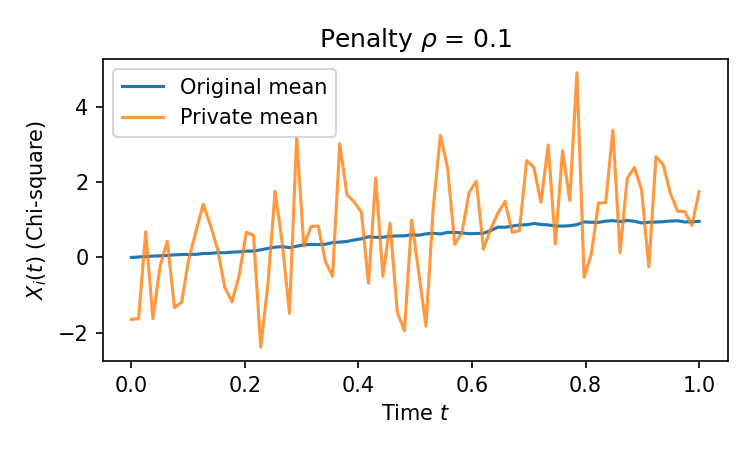
\includegraphics[width=\columnwidth]{fig/fig8.png}
	\caption{Additional experiment (see text).}\label{fig:fig8}
\end{figure}
Figure~\ref{fig:fig8} provides a further experimental result. It can be used to illustrate an extended comparison (e.g., different datasets, parameter sweeps, or ablation) and is included for completeness.

\section{Full multi-dataset validation results}\label{app:multidata}
\begin{table*}[t!]
\centering
\caption{Multi-dataset real-data validation: same entropy+DP pipeline on seven datasets ($\varepsilon=1$, 30 bins; $n$ capped at 100k where applicable).}
\label{tab:csv_entropy_multi}
\begin{tabular}{lrrrrrr}
\hline
Dataset (column) & $n$ & bins & $\varepsilon$ & $H_{\mathrm{orig}}$ & $H_{\mathrm{noisy}}$ & $\Delta_H$ bound \\
\hline
y\_amazon-google-large ($y$) & 100000 & 30 & 1.0 & 3.0279 & 3.0286 & 0.00037 \\
house-prices-train (SalePrice) & 1460 & 30 & 1.0 & 3.4873 & 3.5155 & 0.01676 \\
home-credit-application-train (AMT\_INCOME\_TOTAL) & 100000 & 30 & 1.0 & 0.0004 & 0.0034 & 0.00037 \\
tabular-feature-engineering ($y_1$) & 10000 & 30 & 1.0 & 4.6645 & 4.6640 & 0.00300 \\
r\_diff\_train ($y_1$) & 10000 & 30 & 1.0 & 0.0237 & 0.0459 & 0.00300 \\
pow\_train ($y_1$) & 10000 & 30 & 1.0 & 4.7066 & 4.7065 & 0.00300 \\
unemployment\_data (UNRATE) & 601 & 30 & 1.0 & 4.0457 & 4.0894 & 0.03645 \\
\hline
\end{tabular}
\end{table*}

\begin{figure*}[t!]
	\centering
	\subfigure[Amazon-Google reviews ($y$).]{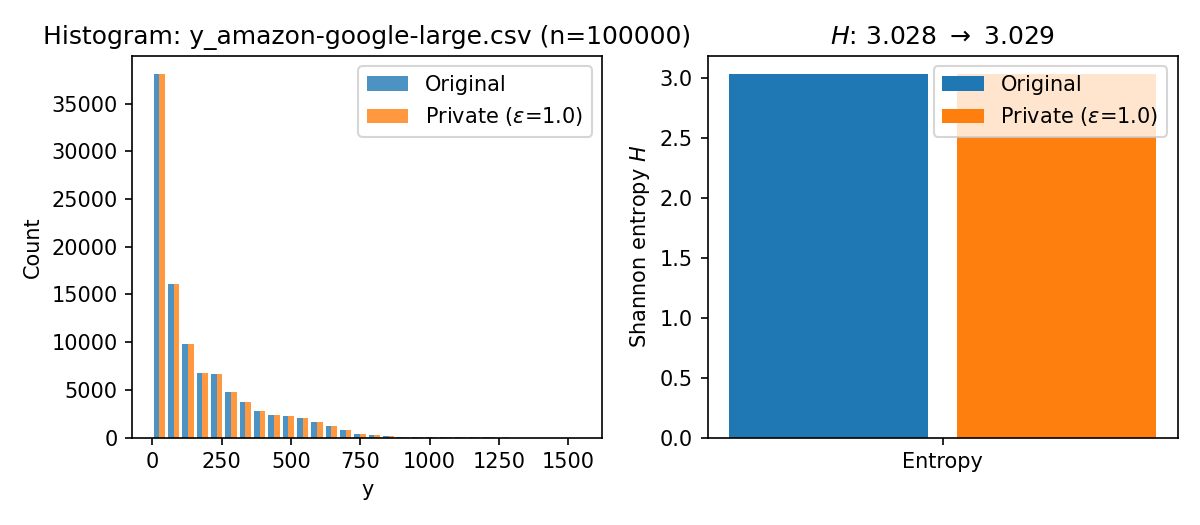
\includegraphics[width=0.48\textwidth]{fig/fig_csv_entropy_y_amazon-google-large.png}}
	\hfill
	\subfigure[House prices (SalePrice).]{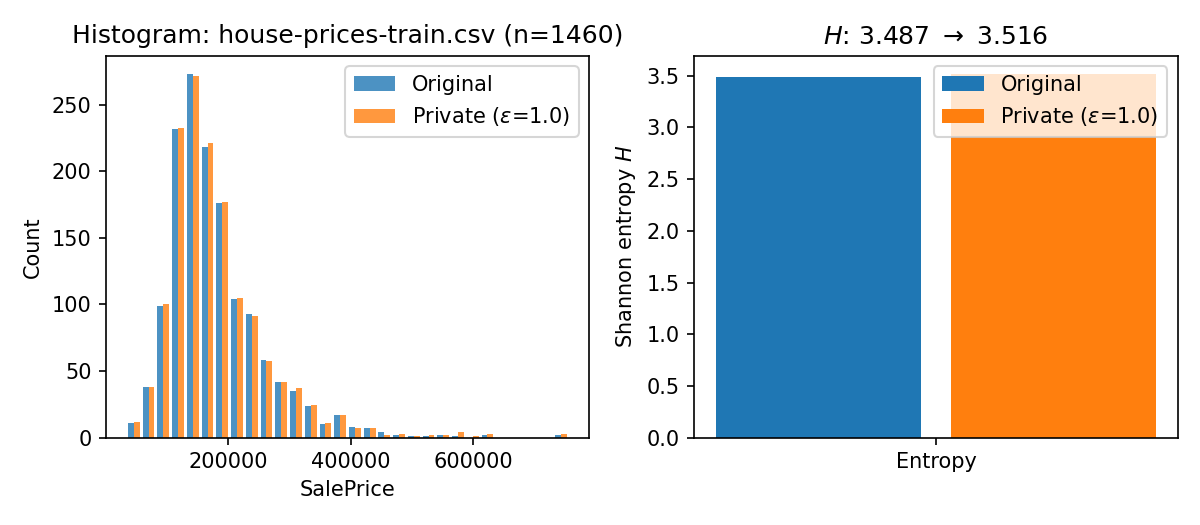
\includegraphics[width=0.48\textwidth]{fig/fig_csv_entropy_house-prices-train.png}}\\
	\subfigure[Tabular feature engineering ($y_1$).]{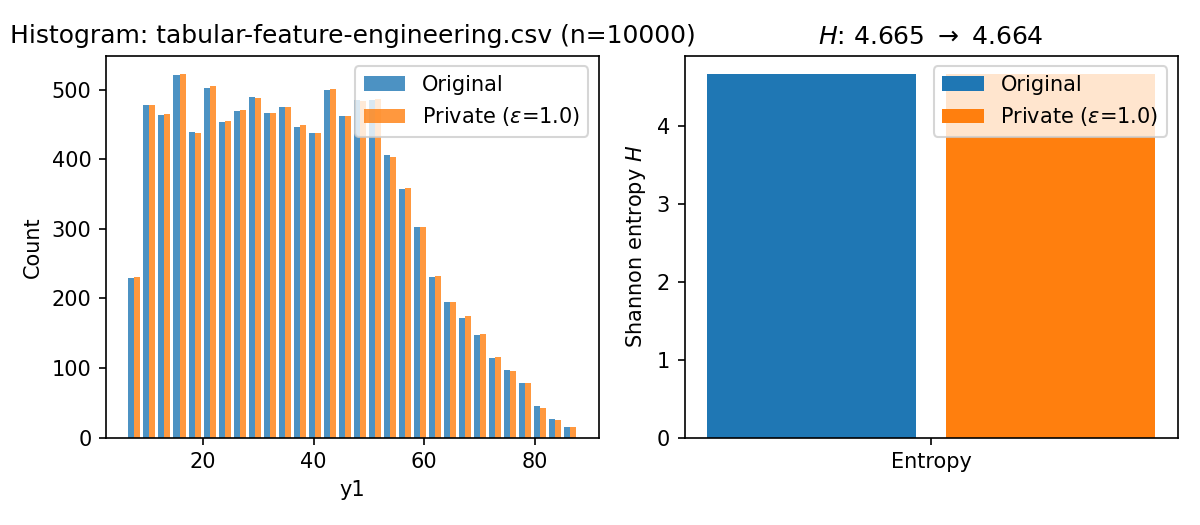
\includegraphics[width=0.48\textwidth]{fig/fig_csv_entropy_tabular-feature-engineering.png}}
	\hfill
	\subfigure[U.S. unemployment (UNRATE).]{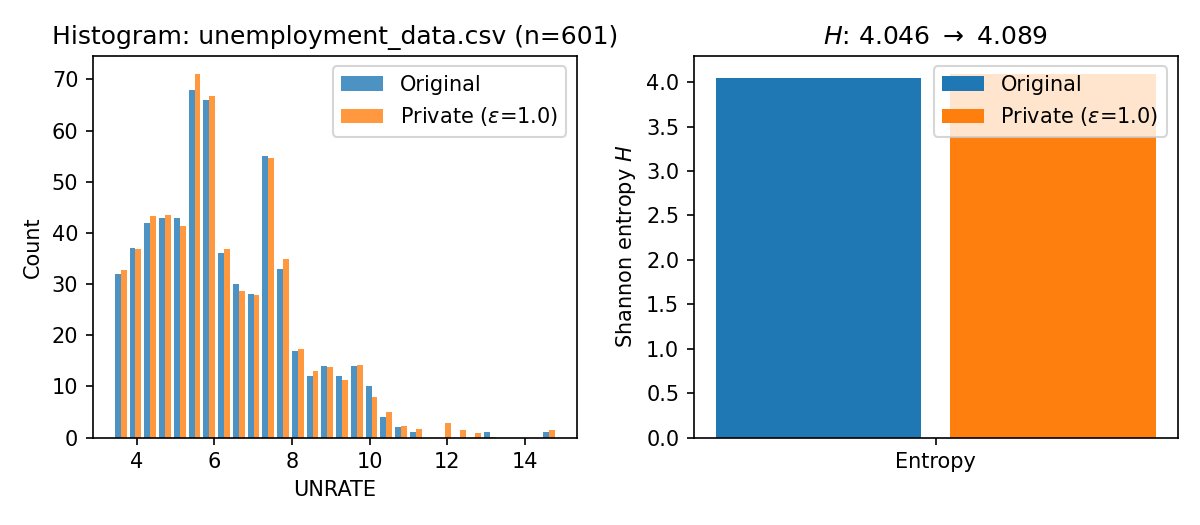
\includegraphics[width=0.48\textwidth]{fig/fig_csv_entropy_unemployment_data.png}}
	\caption{Multi-dataset validation: histogram and entropy (original vs.\ $\varepsilon$-DP) on four representative public datasets. Same mechanism and Theorem~\ref{thm4} bound; full table in Table~\ref{tab:csv_entropy_multi}.}\label{fig:csv_entropy_multi}
\end{figure*}

\bibliographystyle{IEEEtran}
\bibliography{IEEEabrv,ref}
% that's all folks
\end{document}
